\documentclass{beamer}

\usepackage[slovene]{babel}
\usepackage[utf8]{inputenc}
\usepackage[T1]{fontenc}
\usepackage{lmodern}
\usepackage{blindtext}
\usepackage{amsmath} % pravilen izpis v "math mode"
\usepackage{amssymb}
\usepackage{mathtools}
\usepackage{hyperref}
\hypersetup{hidelinks}
\usepackage{amsthm}
\usepackage{graphicx}
\usepackage{fancyhdr}
\usepackage{tcolorbox}
\usepackage{fdsymbol}
\usepackage{bbm}
\usepackage{ascii}
\usepackage[ddmmyyyy]{datetime}
\usepackage{newunicodechar}
\usepackage{subcaption}
\usepackage{makecell}
\usepackage{array}     % določili <{...} in >{...} pri tabelah
\usepackage{tikz}
\usepackage{xcolor}
\usepackage{mathtools}

\usepackage{algorithm,algorithmic}

\newtheorem{primer}{Primer}
\newtheorem{formula}{Formula}
\newtheorem{zgled}{Zgled}
\newtheorem{opomba}{Opomba}
\newtheorem{definicija}{Definicija}
\newtheorem{izrek}{Izrek}
\newtheorem{lema}{Lema}
\newtheorem{trditev}{Trdtev}
\newtheorem{posledica}{Posledica}
\renewcommand{\dateseparator}{.}

\newcommand{\R}{\mathbb R}
\newcommand{\N}{\mathbb N}
\newcommand{\Z}{\mathbb Z}
\newcommand{\C}{\mathbb C}
\newcommand{\Q}{\mathbb Q}
\newcommand{\I}{\mathbbm 1}
\newcommand{\E}{\mathbb E}
\newcommand{\p}{\mathbb P}
\newcommand{\V}{\mathbb{V}\no{ar}}
\newcommand{\e}{\mathcal{E}}
\newcommand{\f}{\mathcal{F}}
\newcommand{\g}{\mathcal{G}}
\newcommand{\h}{\mathcal{H}}
\newcommand{\x}{(X_t)_{t \geq 0}}
\newcommand{\y}{(Y_t)_{t \geq 0}}
\newcommand{\n}{(N_t)_{t \geq 0}}
\newcommand{\s}{(S_t)_{t \geq 1}}
\newcommand{\ff}{(\mathcal{F}_t)_{t \geq 1}}
\newcommand{\vp}{( \Omega ,\mathcal{F}, \p )}
\newcommand{\vph}{( \hat{\Omega},\hat{\mathcal{F}}, \hat{\p })}
\newcommand{\rd}{(\R ^d, \mathcal{B}(\R ^d))}
\newcommand{\no}[1]{\textnormal{#1}}
\newcommand\sbullet[1][.5]{\mathbin{\vcenter{\hbox{\scalebox{#1}{$\bullet$}}}}}




\newcommand{\dis}{\stackrel{\mathclap{\normalfont\mbox{(d)}}}{\simeq}} 




\DeclarePairedDelimiter\ceil{\lceil}{\rceil}
\DeclarePairedDelimiter\floor{\lfloor}{\rfloor}



\usetheme{CambridgeUS}
\usecolortheme{beaver}
% \usecolortheme{orchid}
% \beamertemplatenavigationsymbolsempty


% pisava
\usepackage{palatino}
\usefonttheme{serif}

% definicije in izreki

\begin{document}


% ===================================================================

\title{Diskretne Coonsove ploskve}
\author{Matej Rojec, Vito Rozman}
\date{\today}

\begin{frame}
   \titlepage
\end{frame}

% -------------------------------------------------------------------



% ===================================================================


\begin{frame}
\frametitle{Povzetek}
   \tableofcontents
\end{frame}


% ===================================================================

\section{Uvod}


\begin{frame}
\frametitle{Problem}
\begin{block}{Opis problema}
Podane imamo štiri robne krivulje: 
$$\mathbf{x}(u,0), \mathbf{x}(u,1), \mathbf{x}(0,v),  \mathbf{x}(1,u).$$
\end{block}

\begin{block}{Naloga}
Najti ploskev
$$\mathbf{x}(u,v), (u,v) \in [0,1]^2,$$ 
ki jih interpolira.
\end{block}

\end{frame}


\begin{frame}
    \frametitle{Prevedba v jezik RPGO -- Problem}
    \begin{block}{Problem}
    Podane imamo štiri kontrolne poligone: 
    
    $$
    \begin{matrix}
       \mathbf{b}_{0,0}  &\mathbf{b}_{1,0} & \ldots &\mathbf{b}_{m-1,0} &\mathbf{b}_{m,0} \\
       \mathbf{b}_{0,1}  &                 &        &                   &\mathbf{b}_{m,1} \\
       \vdots            &                 &        &                   &  \vdots\\
       \mathbf{b}_{0,n-1} &                &        &                    &\mathbf{b}_{m,n-1} \\ 
       \mathbf{b}_{0,n}  &\mathbf{b}_{1,n} & \ldots &\mathbf{b}_{m-1,n} &\mathbf{b}_{m,n} 
    \end{matrix}
    $$
          
\end{block}
    
\begin{block}{}
    $\mathbf{b}_{i,j}$ pripada domenskem parametru $\left( \frac{i}{m}, \frac{j}{n}  \right)$          
\end{block}


\end{frame}

\section{Coonosove ploskve}

\begin{frame}
    \frametitle{Prevedba v jezik RPGO -- Problem}
\begin{block}{Ti določajo štiri Bézierjev krivulje}
    \begin{align*}
        &\mathbf{p}(u,0) =\sum_{i=0}^m \mathbf{b}_{i,0} B_i^m(u), \qquad
        \mathbf{p}(u,1) =\sum_{i=0}^m \mathbf{b}_{i,n} B_i^m(u),  \\
        &\mathbf{p}(0,v) =\sum_{j=0}^n \mathbf{b}_{0,j} B_j^n(v), \qquad
        \mathbf{p}(1,v) =\sum_{j=0}^n \mathbf{b}_{m,j} B_j^n(v),  \\
    \end{align*}    
    nad domeno $(u,v) \in [0,1]^2.$
\end{block}



\end{frame}



\begin{frame}
    \frametitle{Coonosove ploskve -- ideja}
    \begin{block}{Določitev točk}
    
    $$
    \begin{matrix}
        \color{blue} \mathbf{b}_{0,0}  &\mathbf{b}_{1,0} & \ldots & \color{red} \mathbf{b}_{i,0} & \ldots &\mathbf{b}_{m-1,0}  &\color{blue} \mathbf{b}_{m,0} \\
       \mathbf{b}_{0,1}  &                 &        & &      &                   &\mathbf{b}_{m,1} \\
       \vdots            &                 &        & &     &                   &  \vdots\\
       \color{red} \mathbf{b}_{0,j}                 &                 &        & \mathbf{b}_{i,j} &  &   & \color{red} \mathbf{b}_{m,j} \\                  &  \\
       \vdots            &                 &        & &    &                   & \vdots \\
       \mathbf{b}_{0,n-1} &                &         & &     &                    &\mathbf{b}_{m,n-1} \\ 
       \color{blue} \mathbf{b}_{0,n}  &\mathbf{b}_{1,n} & \ldots  & \color{red} \mathbf{b}_{i,n} & \ldots  &\mathbf{b}_{m-1,n} &\color{blue} \mathbf{b}_{m,n} 
    \end{matrix}
    $$
\end{block}
    
\end{frame}

\begin{frame}
    \frametitle{Coonosove ploskve -- eksplicitno}
    \begin{block}{Določitev točk}
    
        \begin{align*}
            \mathbf{b}_{i,j} &= \left(1 - \frac{i}{m}\right) \color{red} \mathbf{b}_{0,j} \color{black}+\frac{i}{m}\color{red}\mathbf{b}_{m,j}\\
             &+ \left(1 - \frac{j}{n}\right)\color{red}\mathbf{b}_{i,0} \color{black}+\frac{j}{n} \color{red}\mathbf{b}_{i,n}\ \\
            &- 
            \begin{bmatrix} 
               1 - \frac{i}{m} & \frac{i}{m}
            \end{bmatrix}
            \begin{bmatrix} 
                \color{blue} \mathbf{b}_{0,0} &  \color{blue} \mathbf{b}_{0,1}\\
                \color{blue} \mathbf{b}_{1,0} &  \color{blue} \mathbf{b}_{1,1}
            \end{bmatrix}
            \begin{bmatrix}
               1 - \frac{j}{n}\\
               \frac{j}{n}
            \end{bmatrix}
         \end{align*}
\end{block}
    

\begin{block}{Definicija -- Coonsova ploskev}
    Ploskev, ki jo dobimo s tako dobljenimi kontrolnimi točkami $\mathbf{b}_{i,j}$
imenujemo Coonsova ploskev.

\end{block}

\end{frame}


\begin{frame}
    \frametitle{Coonosove ploskve -- primer}
    Primer okvirja in kontrolnih točk Cossonove krivulje
	\begin{columns}[c]
		\begin{column}{0.5\textwidth}
			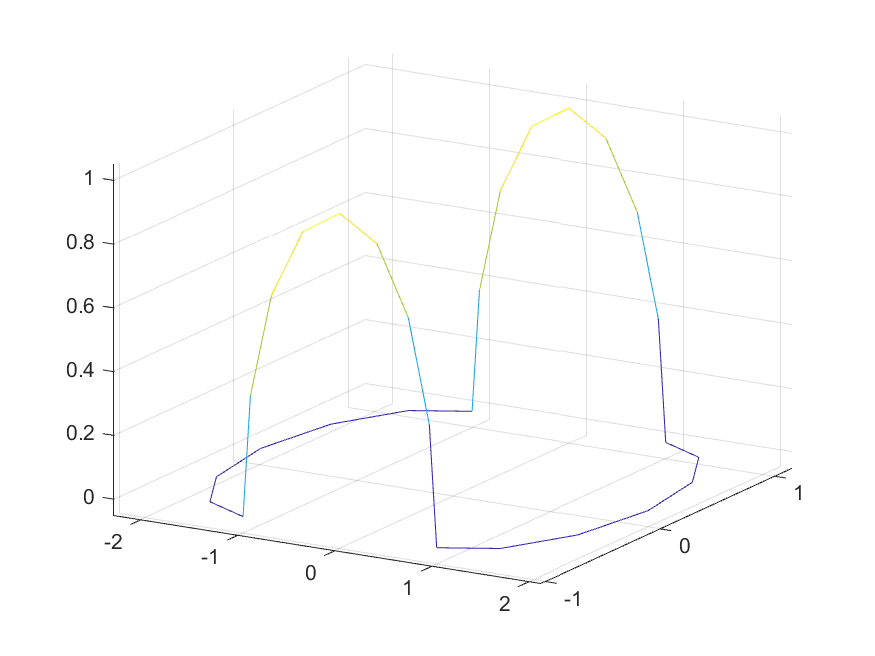
\includegraphics[width=0.98\textwidth]{ogrodje.png}
		\end{column}
		\begin{column}{0.5\textwidth}
			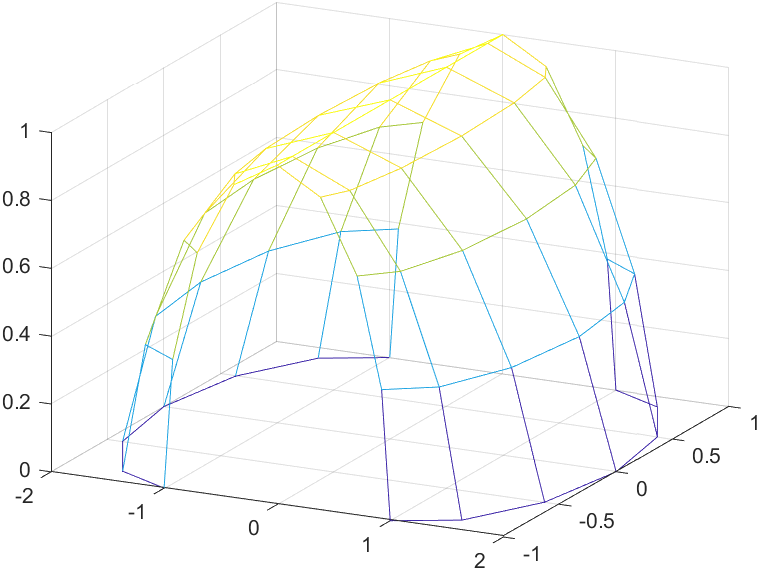
\includegraphics[width=0.98\textwidth]{dodatne_kont_t.png}
		\end{column}
	\end{columns}
\end{frame}

\begin{frame}
    \frametitle{Coonosove ploskve -- primer}
    Primer Cossonove krivulje
    \begin{figure}
        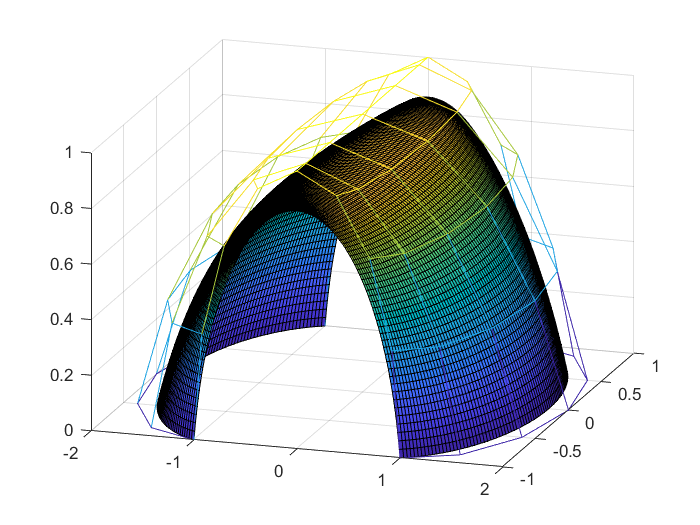
\includegraphics[width=0.8\textwidth]{primer_krivulje.png}
    \end{figure}
\end{frame}

\section{Stalnost Coonosove ploskve}

\begin{frame}
    \frametitle{Ideja}
\begin{block}{Stalnost}
    \begin{itemize}
        \item     Izberemo dve točki $(u_0,v_0)$ in $(u_1,v_1)$ ki razpenjata pravokotnik $R$ v domeni $D =  [0,1]^2$. 
        \item  Štiri mejne pod-Coonosove ploskve se preslikajo na prvotno Coonosovo ploskev
    \end{itemize}
\end{block}

\begin{block}{To načelo lahko uporabimo na diskretni $3 \times 3$ Coonsovi ploskivi:}
    $$
\begin{matrix} 
   \mathbf{b}_{i-1,j-1} & \mathbf{b}_{i-1,j} & \mathbf{b}_{i-1,j+1}\\
   \mathbf{b}_{i,j-1} & \mathbf{b}_{i,j} & \mathbf{b}_{i,j+1}\\
   \mathbf{b}_{i+1,j-1} & \mathbf{b}_{i+1,j} & \mathbf{b}_{i+1,j+1}
\end{matrix}
    $$ 
\end{block}
\end{frame}

\begin{frame}
\frametitle{Računanje točk s pomočjo Coonosove ploskve}
Če poznamo robne točke lahko notranjo točko $\mathbf{b}_{i,j}$ določimo na sledeč način: 
\begin{block}{Točke}

    \begin{align*}
        \mathbf{b}_{i,j} =& -\frac{1}{4}(\mathbf{b}_{i-1,j-1} + \mathbf{b}_{i+1,j-1} +
           \mathbf{b}_{i-1,j+1} + \mathbf{b}_{i+1,j+1}) \\
           &+\frac{1}{2}(\mathbf{b}_{i-1,j} + \mathbf{b}_{i,j-1}+
           \mathbf{b}_{i,j+1} + \mathbf{b}_{i+1,j}).\\
     \end{align*}
     Sistem $(m+1)\times(n+1)$ linearnih enačb
\end{block}
\end{frame}

\begin{frame}
\frametitle{Stalne ploskve}
\begin{block}{Coonosova maska}
    $$
    \mathbf{b}_{i,j} = \frac{1}{4} \times 
    \begin{matrix*}[r]
    -1 && 2 && -1 \\
    2 && \sbullet && 2\\
    -1 && 2 && -1
    \end{matrix*}
    $$
\end{block}

\begin{block}{Splošna tenzorska maska}
    $$
    \mathbf{b}_{i,j} =  \quad 
    \begin{matrix*}[r]
    \alpha && \beta && \alpha \\
    \beta && \sbullet && \beta \\
    \alpha && \beta && \alpha
    \end{matrix*}
    $$
    Afinost: $4\alpha + 4\beta = 1$
\end{block}

\begin{block}{Coonosova maska}
    $(\alpha, \beta) = (-0.25, 0.5)$
\end{block}
\end{frame}


\begin{frame}
    \frametitle{Stalne ploskve -- primer}
    Stalni krivulji pridobljeni s parametroma $\alpha = -0.26$ (leva) in $\alpha = -0.23$ (desna slika)
    \begin{columns}[c]
		\begin{column}{0.5\textwidth}
			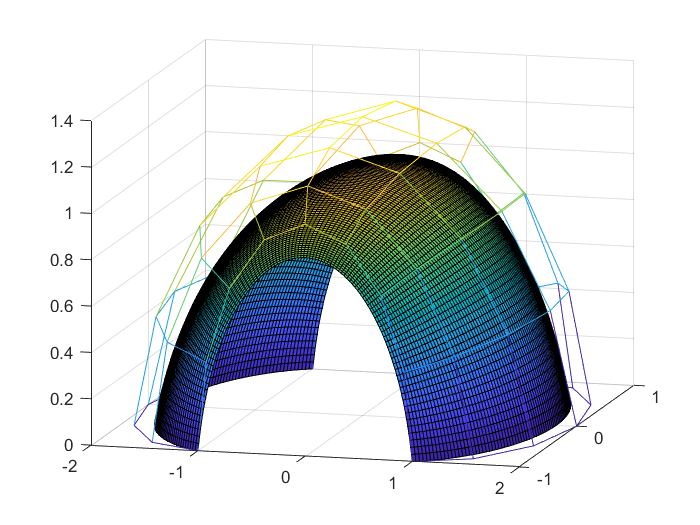
\includegraphics[width=0.98\textwidth]{square_26.png}
		\end{column}
		\begin{column}{0.5\textwidth}
			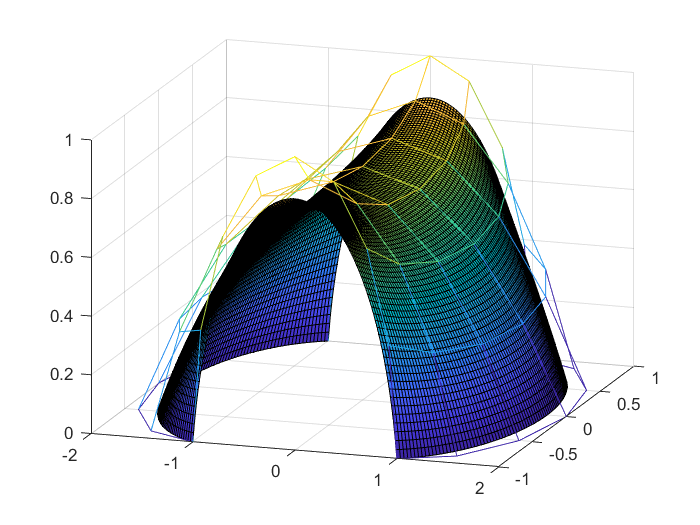
\includegraphics[width=0.98\textwidth]{square_23.png}
		\end{column}
	\end{columns}
\end{frame}

\begin{frame}
    \frametitle{Stalne ploskve -- primer}
    Stalna krivulja pridobljena s parametrom $\alpha = 0$ 
    \begin{figure}
        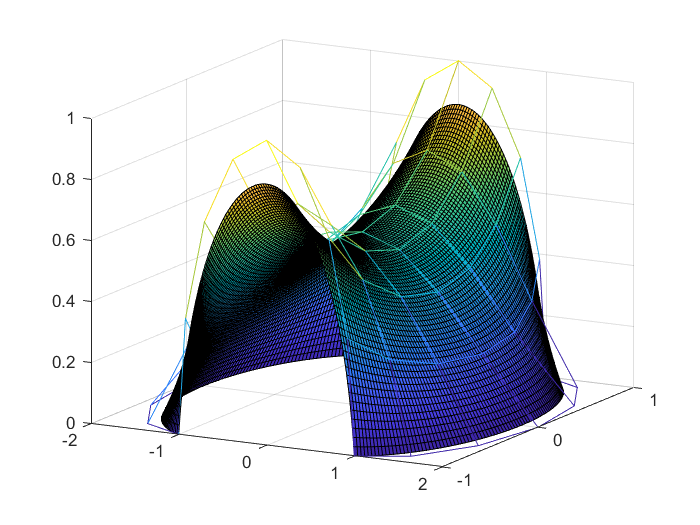
\includegraphics[width=0.8\textwidth]{square_0.png}
    \end{figure}
\end{frame}


\section{Trikotne stalne ploskve}


\begin{frame}
    \frametitle{Trikotna maska}
    \begin{block}{Maska}
    $$
    \mathbf{b}_{\mathbf{i}} =  \quad 
    \begin{matrix*}[r]
            &       &       & \alpha   &       &       & \\
            &       & \beta &          & \beta &       & \\
            & \beta &       & \sbullet &       & \beta & \\
    \alpha &       & \beta &          & \beta &       & \alpha
    \end{matrix*}
    $$
    Rešimo sistem $\binom{m+1}{2}$
    linearnih enačb, kjer je $m$ število kontrolnih točk 
    na eni stranici trikotnika

    Afinost: $3\alpha + 6\beta = 1$
    \end{block}
\end{frame}


\begin{frame}
    \frametitle{Stalne trikotne krpe -- primer 1}
    Stalni krivulji pridobljeni s parametroma $\alpha = 0$ (leva) in $\alpha = -1/6$ (desna slika)
    \begin{columns}[c]
		\begin{column}{0.5\textwidth}
			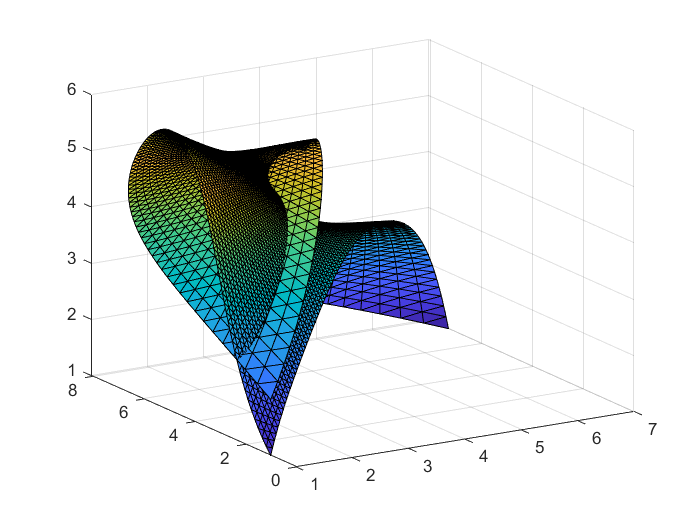
\includegraphics[width=1.2\textwidth]{trikotne_0.png}
		\end{column}
		\begin{column}{0.5\textwidth}
			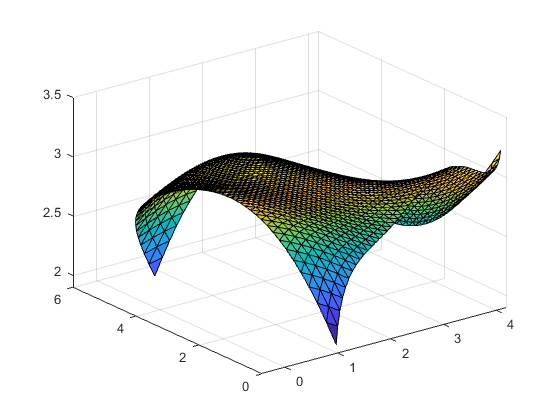
\includegraphics[width=1.2\textwidth]{trikotne_1_6.png}
		\end{column}
	\end{columns}
\end{frame}

\begin{frame}
    \frametitle{Stalne trikotne krpe -- primer 2}
    Stalna krivulja pridobljena s parametrom $\alpha = -1/9$ 
    \begin{figure}
        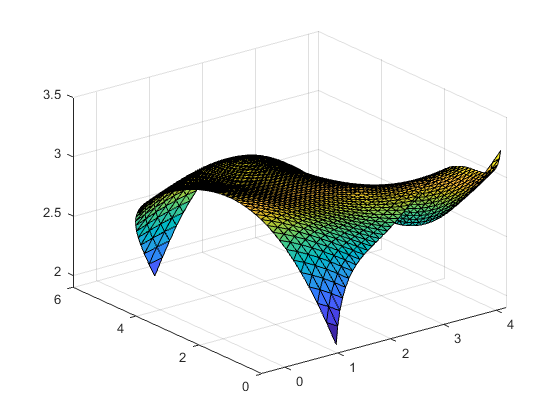
\includegraphics[width=0.8\textwidth]{trikotne_1_9.png}
    \end{figure}
\end{frame}

\end{document}